\section{Feedback}
\exercise{Grundlagen}
Beantworte die folgenden Fragen
\begin{itemize}
    \item Welche Formen von Feedback gibt es?
    \item Was können biologische Mechanismen für Feedback sein? Finde mindestens ein Beispiel zu zellulären, makroskopischen und globalen Prozessen (die noch nicht in der Vorlesung genannt wurden).
    \item 
\end{itemize}
%
%
\exercise{Feedback Loops}
Gegeben sind verschiedene \acp{ode} zu biologischen Systemen.
\begin{enumerate}
    \item Analysiere die Systeme qualitativ auf positives/negatives Feedback
    \item Können wir die Systeme in Bezug auf Feedback loops vereinfachen?
    \item Welches qualitative Verhalten können wir erwarten?
    \item Gibt es einen Gleichgewichtszustand?
\end{enumerate}
\begin{equation}
    \dot{A} = k_0 - k_1 A
\end{equation}
%
\begin{equation}
    \begin{aligned}
        \dot{A} &= k_0 + k_1 \frac{A^2}{B} - k_2a\\
        \dot{B} &= k_3 + k_1 A^2 - k_4 B
    \end{aligned}
\end{equation}
%
\begin{equation}
    \begin{aligned}
        \dot{s} &= -&&k_1se &&+ k_{-1}c\\
        \dot{e} &= -&&k_1se &&+ (k_{-1}+k_2)c\\
        \dot{c} &= &&k_1se &&- (k_{-1}+k_2)c\\
        \dot{p} &= &&k_2c
    \end{aligned}
\end{equation}
%
\section{Kontrolltheorie}
\exercise{Grundlagen}
\begin{itemize}
    \item Was ist der Unterschied zwischen Open-Loop and Closed-Loop Control?
    \item Welche Controller gibt es?
    \item Für was sind diese Kontroller jeweils gut? (Wo liegen ihre Stärken/Schwächen?)
    \item Welche Probleme können auftreten?
\end{itemize}
%
\exercise{Python Controller}
\begin{enumerate}
    \item Programmiere in Python folgende Controller
    \begin{enumerate}
        \item P-Controller
        \item I-Controller
        \item D-Controller
        \item Alle Kombinationen der oberen
    \end{enumerate}
    \item Teste die Controller an dem Skript \texttt{bacteria\_growth.py}.
    \begin{enumerate}
        \item Was macht das Skript überhaupt?
        \item Verwende die bereitgestellte Vorlage \texttt{control\_example.py} für dein weiteres Vorgehen.
        Lasse \texttt{bacteria\_growth.py} unverändert.
    \end{enumerate}
\end{enumerate}
%
%
\exercise{Perturbationen}
Verwende die Controller und das zuvor bearbeitete System, um das Verhalten unter Perturbationen zu untersuchen.
Mögliche Ereignisse
\begin{enumerate}
    \item Einmaliges plötzliches Verschwinden von Nährstoffen
    \item Mehrmaliges (randomisiertes) Verschwinden von Nährstoffen
    \item Mehrmaliges periodisches Verschwinden von Nährstoffen
\end{enumerate}
% \exercise{Python erstes Beispiel}
% Das python-script "Bifurkationen.py" bietet eine erste einfache Möglichkeit, Bifurkationen zu plotten.
% Es ist noch leicht unvollständig.
% Verstehe das Skript und vervollständige es.
% Das Endergebnis sollte dann aussehen wie in Figur~\ref{fig:bifurcation-plot}.
% \begin{figure}[!h]
%     \centering
%     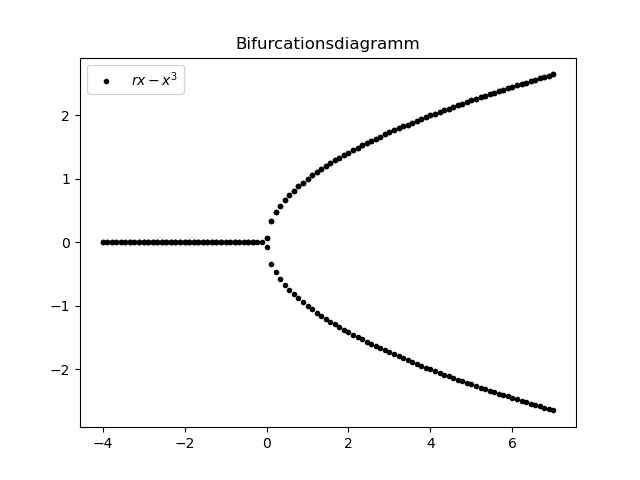
\includegraphics[width=0.6\textwidth]{media/Bifurkationsplot.png}
%     \caption{Bifurkation geplottet mit python}
%     \label{fig:bifurcation-plot}
% \end{figure}
% %
% %
% \exercise{Auf Papier: Erwartungen an Systeme}
% Betrachte die folgenden Gleichungen jeweils als einzelstehende \acp{ode}. Welche davon zeigen Bifurkationen? Welche weiteren Verhaltensweisen sind zu erwarten? Wie viele Gleichgewichtszustände gibt es?
% \begin{align}
%     \dot{x} &= -rx^3+x\\
%     \dot{x} &= x - rx^3\\
%     \dot{x} &= ax + bx^2 - rx^3\\
%     \dot{x} &= -(x-r)(x-1+r)^2 - (x-r)^2(x-1+r)\\
%     \dot{x} &= -\frac{\partial}{\partial x}\left(1-\e(-(x-r)^2)\right)^2\left(1-\e(-(x-1+r)^2)\right)^2\\
%     \dot{x} &= -\frac{\partial V}{\partial x}(x)
% \end{align}
% wobei $g(x)$ gegeben ist durch Diagramme aus Figur~\ref{fig:potential-plots}.
% \begin{figure}[!h]
%     \centering
%     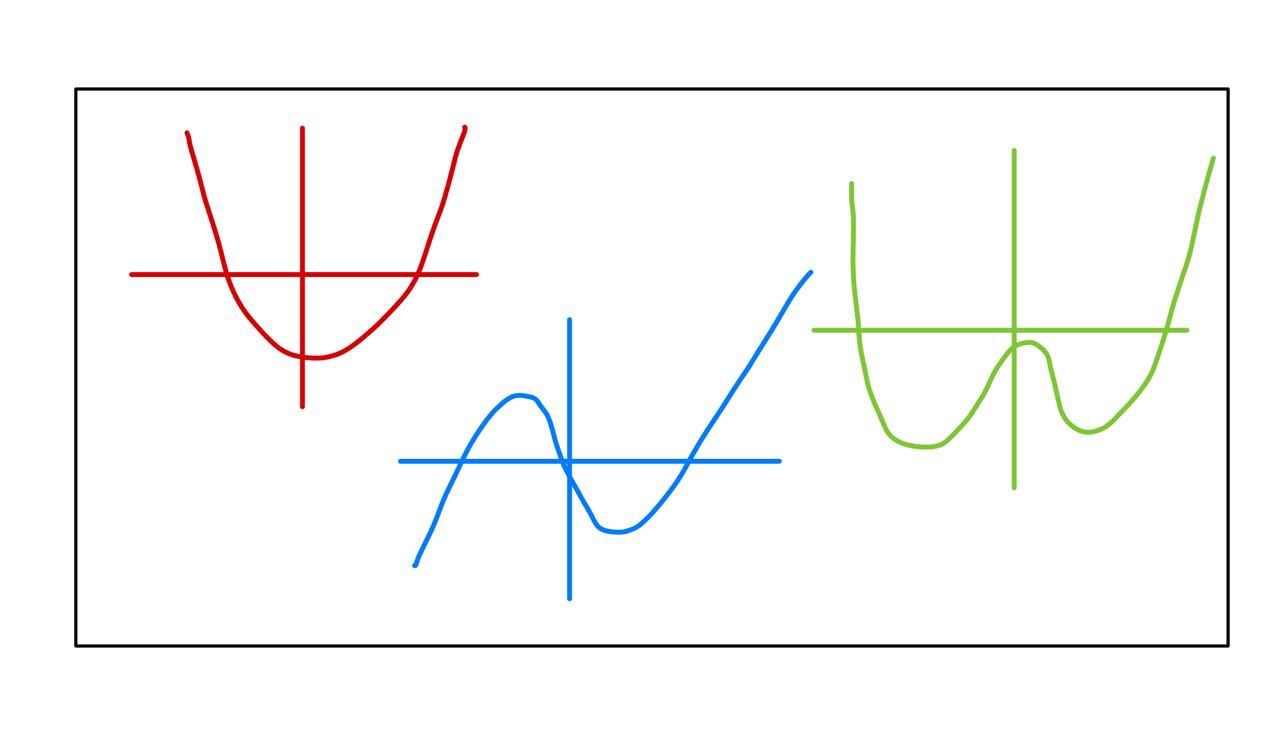
\includegraphics[width=0.75\textwidth]{media/potential-plots.jpg}
%     \caption{Plots für Möglichkeiten von $V(x)$.}
%     \label{fig:potential-plots}
% \end{figure}
% %
% %
% \exercise{Erwartungen überprüfen}
% Benutze das python-script von zuvor, um die oben beschriebenen Systeme zu plotten und mit deinen Erwartungen zu vergleichen.
% %
% %
% \exercise{Hopf-Bifurkation (Zusatz)}
% Wie müsste man das vorheregangene Muster verändern, um eine Hopf-Bifurkation zu visualisieren?
% Schreibe ein Python-script für die folgende \ac{ode}
% \begin{align}
%     \dot{x} &= \lambda(x+y) + \alpha(x^2+y^2)\\
%     \dot{y} &= x+y+\beta(x^2+y^2)
% \end{align}
% Für welche Werte von $\lambda,\alpha,\beta$ finden wir Bifurkationen, stabile Fixpunkte etc.?
% %
% %
% \section{Toggle-Switch Model}
% %
% %
% \exercise{Grundlagen}
% Beantworte die folgenden Fragen zum Toggle-Switch model
% \begin{align}
%     \dot{A} &= \frac{a_1}{1+B^n} - A\\
%     \dot{B} &= \frac{a_2}{1+A^n} - B
% \end{align}
% \begin{itemize}
%     \item Gehört dieses System von \acp{ode} zu einer Reaktion, die wir aufschreiben können?
%     \item Was möchte man mit diesem mathematischen model biologisch simulieren?
%     \item Was ist eine Nullcline? Warum ist sie hilfreich?
% \end{itemize}
% %
% %
% \exercise{Nullclinen}
% Berechne die Nullclinen von Hand.
% Schreibe ein Python script, welches die Nullclinen numerisch berechnet und plottet.
% Vergleiche die Ergebnisse mit deinen Berechnungen von Hand.
% Was kann man von den plots ablesen?
% Welche Schlüsse lassen sich ziehen?
% %
% %
% \exercise{Flussdiagramm}
% Das python script "Toggle-Switch-Fluss.py" wurde bereits im Vorhinein angelegt.
% Mache dich mit dem Skript vertraut und versuche zu verstehen, was in den einzelnen Schritten passiert.
% Finde einen Satz von parametern $a_1,a_2,n$, sodass ein Schaubild wie das aus Figur~\ref{fig:toggle-switch-flowdiag} zustande kommt.
% Beantworte die folgenden Fragen
% \begin{itemize}
%     \item Was sehen wir auf dem Plot?
%     \item Wie hilft uns das in der Analyse?
%     \item Was können wir nicht sehen?
% \end{itemize}
% Benutze dein Ergebnis für die geplotteten nullclinen und füge diese dem plot hinzu.
% Macht es Sinn, das in einen plot zu kombinieren?
% Was zeigt uns das resultierende Schaubild?
% \begin{figure}[!h]
%     \centering
%     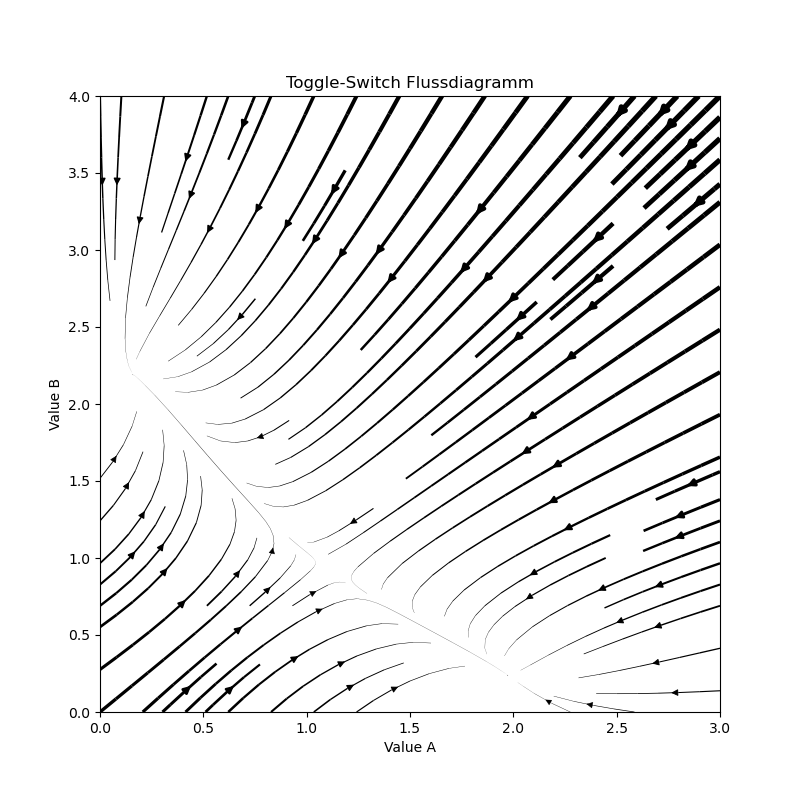
\includegraphics[width=0.7\textwidth]{media/Toggle-Switch-Fluss.png}
%     \caption{Flussdiagramm des Toggle-Switch Models}
%     \label{fig:toggle-switch-flowdiag}
% \end{figure}
% %
% %